\documentclass{llncs}

\usepackage[T1]{fontenc}
\usepackage[utf8]{inputenc}
\usepackage{graphicx}
\usepackage{amsmath,amssymb}
\usepackage{booktabs}
\usepackage{cite}
\usepackage{siunitx}
\usepackage{xcolor}
\usepackage[hidelinks]{hyperref}

\sisetup{group-digits=none, table-number-alignment=center}
\renewcommand\UrlFont{\color{blue}\rmfamily}

\begin{document}

\title{One-to-one SkewGRAM: Applying NLP Embeddings to Biological Graph Optimization}
\titlerunning{One-to-one SkewGRAM: NLP Embeddings for Biological Graphs}

\author{Bechir Mady\inst{1} \and
Abderahmane Abderrahmane\inst{1} \and
Mohamedou Yahya Cheikh Mohamed Vall\inst{1} \and
El Moustapha Mohamed El Moustapha\inst{1} \and
Mohamed Lemine Ahmed Sidi\inst{1} \and
Hafedh Mohamed Babou\inst{2}}
\authorrunning{B. Mady et al.}

\institute{Unité de Recherche en Systèmes Intelligents Avancés (URSIA), Institut Supérieur du Numérique (SupNum), Nouakchott, Mauritania\\
\email{\{22014,22053,25239,22013\}@supnum.mr, m-lamine.ahmed-sidi@supnum.mr}
\and
École Supérieure Polytechnique (ESP), Nouakchott, Mauritania\\
\email{hafedh.mohamed-babou@esp.mr}}

\maketitle

\begin{abstract}
The One-to-one SkewGRAM problem asks for a longest path in a directed acyclic graph $D$ whose vertices induce a connected subgraph in an undirected graph $G$ defined on the same vertex set. It arises when metabolic pathways are compared with genomic or functional networks, and it is NP-hard. The exact ILP2 model needs tens of seconds on 100-vertex instances and minutes on 200-vertex ones, while earlier graph neural network decoders return paths of about one vertex. Our method, Skew-GRAM, borrows the Skip-Gram model from natural language processing: directed random walks on $D$ are read as sentences, and vertex embeddings are learned with negative samples drawn from non-successors. A Monte-Carlo decoder combines these embeddings with an exact dynamic-programming lookahead on $D$ and a bonus for vertices adjacent in $G$ to the current path. A final Union-Find step extracts the longest sub-path that is connected in $G$, so every returned path is feasible. Over five random seeds on 368 Erd\H{o}s--Rényi instances with an ILP2 solution, the method reaches the ILP2 path length in 71.3\,\% of the runs with 100 vertices and in 30.0\,\% with 200 vertices, with median speedups over ILP2 of 4.0$\times$ and 21.2$\times$; on one 200-vertex instance it finds a longer path than the reported ILP2 solution. It finds the exact optimum on all 25 KEGG metabolic pathways and handles 1000-vertex graphs in about 143 seconds. Without the dynamic-programming lookahead, the paths are 23\,\% shorter on 100-vertex instances.

\keywords{Combinatorial optimization \and Bioinformatics \and Node embeddings \and Skip-Gram \and Dynamic programming \and Union-Find.}
\end{abstract}

% ============================================================
\section{Introduction}
% ============================================================

Biological systems are naturally described as networks whose vertices are biological entities and whose edges are relations between them. Comparing two networks built on the same entities can reveal patterns that neither network shows alone. Metabolism, for instance, is a directed network in which reactions follow each other along pathways, while genomic proximity or protein--protein interactions give an undirected network of functional associations~\cite{sharan2006,zaharia}. A chain of reactions whose genes are also close to each other on the genome is a candidate for a conserved functional unit.

The \emph{One-to-one SkewGRAM} problem formalizes this search~\cite{fertin2012,sidi2022}. Given a directed acyclic graph $D$ and an undirected graph $G$ on the same vertex set, it asks for a longest directed path of $D$ whose vertices induce a connected subgraph of $G$. The problem is NP-hard~\cite{fertin2012,sidi}. Its difficulty comes from the interaction of the two constraints: a valid successor in $D$ may break connectivity in $G$, and vertices that are close in $G$ need not lie on a common path of $D$.

Exact methods solve the problem to optimality. The integer linear program ILP2~\cite{sidi2022,sidi} needs about 30 seconds on 100-vertex instances and about four minutes on 200-vertex instances of our benchmark. Learning-based approaches have also been studied~\cite{sidi_dl}: a dual graph convolutional network with heuristic post-processing, and a graph encoder with an LSTM-attention decoder (DL2). Their sequential decoding produces very short paths, about 1.2 vertices on average for DL2.

This paper takes a different route, from natural language processing (NLP) to biology. Our method, Skew-GRAM, reads directed random walks on $D$ as sentences and learn vertex embeddings with the Skip-Gram model~\cite{mikolov}, as DeepWalk and node2vec do for graphs~\cite{perozzi,grover}. The embeddings alone do not solve the optimization problem, so we use them as one of three signals in a decoder designed for the problem, next to an exact dynamic-programming lookahead on $D$ and a soft connectivity signal from $G$. An exact extraction step then enforces the connectivity constraint.

Our contributions are:
\begin{enumerate}
\item a Skip-Gram embedding model for the vertices of a DAG, trained on directed random walks with hub sub-sampling and structural negative sampling;
\item a guided decoder that combines an exact longest-path lookahead on $D$, embedding similarity and a $G$-connectivity bonus, followed by an exact Union-Find extraction that guarantees feasibility;
\item an evaluation on 375 synthetic instances with 100 and 200 vertices (368 with an ILP2 solution) over five random seeds, on 15 larger instances with 500 and 1000 vertices, and on 25 real metabolic pathways from KEGG~\cite{kanehisa2000} with exact optima, together with an ablation of the lookahead.
\end{enumerate}

% ============================================================
\section{Related Work}
% ============================================================

The One-to-one SkewGRAM problem belongs to a family of problems that compare heterogeneous biological networks, such as the search for metabolic and genomic patterns in CoMetGeNe~\cite{zaharia} and network comparison methods surveyed in~\cite{sharan2006}. Fertin et al.~\cite{fertin2012} studied its complexity and gave exact algorithms for it. Ahmed Sidi et al.\ proposed the integer linear programs ILP1 and ILP2~\cite{sidi2022} and constraint programming models~\cite{sidi}; ILP2 is the exact reference used in this paper.

Learning methods for combinatorial optimization on graphs include pointer networks~\cite{vinyals2015}, reinforcement learning of construction policies~\cite{bello2016,dai2017} and unsupervised training of graph neural networks~\cite{karalias2020}. These models are trained across many instances and then decode a solution. The deep learning approaches of~\cite{sidi_dl} follow this scheme for our problem. Our model is trained on each instance separately, because vertex identifiers carry no shared meaning across independently generated graphs, and the learned embeddings only guide a search whose feasibility is enforced exactly. The embedding model itself follows word2vec~\cite{mikolov} and its graph versions DeepWalk~\cite{perozzi} and node2vec~\cite{grover}.

% ============================================================
\section{Problem Formulation}
% ============================================================

Let $V$ be a set of $n$ biological entities, $D=(V,A)$ a directed acyclic graph that models a causal or sequential relation, and $G=(V,E)$ an undirected graph that models functional association. A path $P=(p_1,\ldots,p_k)$ is \emph{$(D,G)$-consistent} if
\begin{equation}
(p_i,p_{i+1})\in A \quad (i=1,\ldots,k-1) \qquad\text{and}\qquad G[\{p_1,\ldots,p_k\}] \text{ is connected}.
\end{equation}
The goal is to find a $(D,G)$-consistent path with the largest number of vertices. Fig.~\ref{fig:problem} shows a small instance.

\begin{figure}[t]
\centering
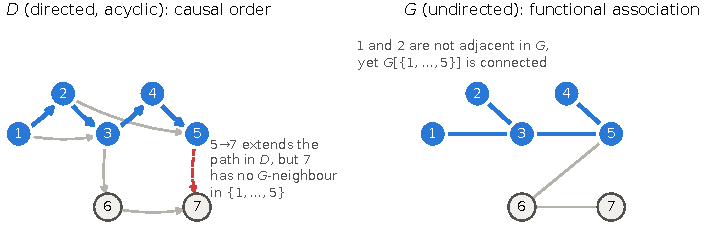
\includegraphics[width=\textwidth]{fig1_problem.pdf}
\caption{Toy instance on seven vertices. The highlighted path $1\to2\to3\to4\to5$ is the unique optimum. Extending it by the arc $5\to7$ gives the longest path of $D$, but vertex 7 has no neighbour in $G$ among the other path vertices. The prefix $(1,2)$ is disconnected in $G$ although the full path is connected.}
\label{fig:problem}
\end{figure}

\subsubsection{Connectivity cannot be checked incrementally.}
\label{sec:incremental}
The connectivity constraint is global. Two consecutive vertices of a feasible path need not be adjacent in $G$, and a prefix of a feasible path can be disconnected in $G$ while the full path is connected (Fig.~\ref{fig:problem}). This is the common case: in our benchmark, all 368 ILP2 solutions contain two consecutive vertices that are not adjacent in $G$, and 363 of them (98.6\,\%) have a disconnected prefix. A decoder that rejects every extension which disconnects the current prefix could not build most of these solutions. Our decoder uses $G$ only as a soft signal while it builds a path, and checks connectivity exactly once the path is complete.

% ============================================================
\section{Method}
\label{sec:method}
% ============================================================

Skew-GRAM has an encoder, which learns vertex embeddings from $D$ only, and a decoder, which uses $D$, the embeddings and $G$ to build paths (Fig.~\ref{fig:pipeline}). It runs once per instance in four phases. The guiding analogy is taken from NLP: a vertex plays the role of a word, a directed random walk the role of a sentence, and the neighbourhood of a vertex in a walk the role of its context.

\begin{figure}[t]
\centering
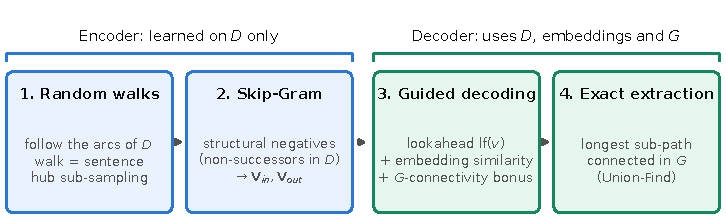
\includegraphics[width=\textwidth]{fig2_pipeline.pdf}
\caption{The four phases of Skew-GRAM, run once per instance. The encoder learns embeddings $\mathbf{V}_{in},\mathbf{V}_{out}$ from walks on $D$; the decoder generates candidate paths (Step~A) and extracts a $(D,G)$-consistent sub-path from each of them (Step~B).}
\label{fig:pipeline}
\end{figure}

\subsubsection{Phase 1: random walks and hub sub-sampling.}
From every vertex with at least one successor, we start several random walks that follow outgoing arcs of $D$: from vertex $u$ the next vertex is drawn uniformly from its successors $N^+(u)$. A walk stops at a sink or at a maximum length. As in word2vec, each occurrence of a vertex $v$ with relative frequency $f(v)$ is kept with probability $\min\bigl(1,\sqrt{t/f(v)}+t/f(v)\bigr)$, $t=10^{-3}$, which reduces the weight of hubs. A sliding window over each walk then yields (centre, context) pairs.

\subsubsection{Phase 2: Skip-Gram embeddings with structural negatives.}
We learn two matrices $\mathbf{V}_{in},\mathbf{V}_{out}\in\mathbb{R}^{n\times d}$. For a centre vertex $c$, a context vertex $o$ and $K$ negative vertices $n_1,\ldots,n_K$, the loss is the usual negative-sampling objective
\begin{equation}
\mathcal{L}(c,o,n_{1:K}) = -\log\sigma(\mathbf{v}_{in,c}^{\top}\mathbf{v}_{out,o}) - \sum_{k=1}^{K}\log\sigma(-\mathbf{v}_{in,c}^{\top}\mathbf{v}_{out,n_k}).
\end{equation}
The difference with standard Skip-Gram lies in how negatives are drawn: instead of a frequency-based distribution, the negatives of $c$ are drawn uniformly among the vertices that are not successors of $c$ in $D$. The negative signal thus reflects the direction of the arcs. The decoder uses the similarity $\operatorname{sim}(u,v)=\mathbf{v}_{in,u}^{\top}\mathbf{v}_{out,v}$.

\subsubsection{Phase 3: guided decoding (Step A).}
A decoder driven by similarity alone tends to pick successors that lead quickly to a sink. We therefore compute, for every vertex $v$, the number $\mathrm{lf}(v)$ of arcs on a longest path of $D$ that starts at $v$:
\begin{equation}
\mathrm{lf}(v) = 0 \ \text{if } N^+(v)=\emptyset, \qquad \mathrm{lf}(v)=\max_{w\in N^+(v)}\bigl(1+\mathrm{lf}(w)\bigr) \ \text{otherwise}.
\end{equation}
Because $D$ is acyclic, all values are obtained in one pass over a reverse topological order, in $O(|V|+|A|)$ time~\cite{bellman1958}. When the current vertex is $u$ and $v\in N^+(u)$ has not been visited yet, the decoder scores $v$ by
\begin{equation}
S(u,v) = \frac{\mathrm{lf}(v)}{\tau_{lf}} + \beta\,\frac{\operatorname{sim}(u,v)}{\tau} + \log(\gamma)\,\mathbb{I}_G(v),
\end{equation}
where $\mathbb{I}_G(v)=1$ if $v$ is adjacent in $G$ to a vertex of the current path and $0$ otherwise. The next vertex is drawn with probability $P(v\mid u)\propto\exp S(u,v)$. The three terms measure the remaining path potential in $D$, the learned compatibility between $u$ and $v$, and a preference for vertices connected in $G$ to the path built so far. Visited vertices are masked. The decoder repeats such walks $W$ times from uniformly chosen start vertices.

\subsubsection{Phase 4: exact extraction (Step B).}
A candidate path $P=(p_1,\ldots,p_L)$ from Phase~3 is a path of $D$ but may be disconnected in $G$. Every contiguous sub-path of $P$ is still a path of $D$, so it suffices to find the longest interval $[i,j]$ such that $G[\{p_i,\ldots,p_j\}]$ is connected. For each start $i$, we extend the window one vertex at a time and maintain the components of the window in a Union-Find structure~\cite{tarjan1975}, comparing each new vertex with the vertices already in the window. This costs $O(L^3\alpha(L))$ for a path of length $L$, where $\alpha$ is the inverse Ackermann function. The extraction is only run when the raw candidate is longer than the best sub-path found so far, and $L$ is bounded by the longest path of $D$ (at most 100 vertices in our instances). The best extracted sub-path over the $W$ walks is returned; by construction it is $(D,G)$-consistent.

% ============================================================
\section{Experiments}
% ============================================================

\subsection{Setup}

\subsubsection{Synthetic instances.}
The main benchmark contains 300 instances with $n=100$ vertices and 75 instances with $n=200$ vertices, each provided with the solution of ILP2 (path and running time). $D$ is built by drawing a random topological order and adding each forward arc with probability $p$ ($p=0.08$ for $n=100$, $p=0.05$ for $n=200$), and $G$ is an independent Erd\H{o}s--Rényi graph $G(n,p)$~\cite{erdos1959}. ILP2 reports no solution for 2 instances with 100 vertices and 5 with 200 vertices; these are excluded from all comparisons with ILP2, which leaves 298 and 70 instances. ILP2 is an exact model, but the reported solutions are not all optimal: on instance 200\_68, Skew-GRAM finds a feasible path with 10 vertices, which we checked independently, while the ILP2 file reports 7. We therefore use the ILP2 solutions as reference lengths and say that a run reaches ILP2 when its path is at least as long. To study scalability we also use 10 instances with $n=500$ and 5 instances with $n=1000$, built in the same way with $p=0.05$ (we generated the 1000-vertex instances ourselves); no ILP2 solution is available for them.

\subsubsection{Real metabolic networks.}
We use 25 metabolic pathways from KEGG~\cite{kanehisa2000}, taken from seven bacteria (KEGG codes aae, bsu, eco, mtv, pae, sau and syn). In each instance, $D$ is the metabolic graph of a pathway and $G$ a graph of genomic or functional proximity on the same vertices. The set contains 19 acyclic pathways (at most three per organism, with 10 to 80 listed entities) and 6 pathways whose only cycles are reversible reactions (2-cycles); vertices without any arc or edge are discarded on loading, which leaves 4 to 38 vertices. Each reversible reaction is oriented from the lower to the higher vertex identifier so that $D$ is acyclic; this is a modelling simplification. These instances have no ILP2 solution, but they are small, so we compute their exact optimum by enumerating the paths of $D$ with two exact cuts: the vertices of a feasible path lie in one connected component $C$ of $G$, so only paths of $D[C]$ are enumerated, and a path ending at $u$ cannot gain more than $\mathrm{lf}(u)$ vertices.

\subsubsection{Protocol.}
Table~\ref{tab:hyper} lists the hyperparameters, which are the same for all instances. Training uses Adam~\cite{kingma2014}. Each instance is solved with five seeds (42 to 46); the seed is reset at the start of each instance, so a result does not depend on the order in which instances are processed. Every returned path is checked to be $(D,G)$-consistent. Skew-GRAM runs on an Intel Core i5-1135G7 laptop processor (4 cores), with four instances solved in parallel and one thread each; the laptop was also used for other work during the runs, so times include some load-related noise. ILP2 times come from the dataset files and were measured on another machine, so speedups are indicative only.

\begin{table}[t]
\centering
\caption{Hyperparameters, identical for all instances.}
\label{tab:hyper}
\begin{tabular}{@{}llr@{\qquad}llr@{}}
\toprule
\multicolumn{3}{@{}l}{Encoder (Phases 1--2)} & \multicolumn{3}{l@{}}{Decoder (Phases 3--4)} \\
\midrule
Walks per start vertex & & 40 & Decoding walks & $W$ & 30{,}000 \\
Maximum walk length & & 30 & Lookahead temperature & $\tau_{lf}$ & 1.5 \\
Context window & & 3 & Similarity temperature & $\tau$ & 0.5 \\
Embedding dimension & $d$ & 32 & Similarity weight & $\beta$ & 0.3 \\
Negatives per pair & $K$ & 5 & $G$-connectivity bonus & $\gamma$ & 6.0 \\
Epochs / learning rate & & 8 / 0.01 & & & \\
\bottomrule
\end{tabular}
\end{table}

\subsection{Comparison with ILP2}
\label{sec:ilp2}

Table~\ref{tab:results} summarizes the results. Values after $\pm$ are standard deviations across the five seeds of the corresponding mean, except for running times, where they are standard deviations over all runs.

\begin{table}[t]
\centering
\caption{Skew-GRAM compared with ILP2 on the synthetic instances with an ILP2 solution (five seeds per instance). ILP2 length reached: runs whose path is at least as long as the ILP2 solution. Speedup: median over instances of the ratio between the ILP2 time and the mean Skew-GRAM time.}
\label{tab:results}
% Généré par scripts/make_paper_assets.py — ne pas modifier à la main.
\setlength{\tabcolsep}{7pt}
\begin{tabular}{@{}l S[table-format=-3.2]@{\,$\pm$\,}S[table-format=1.2] S[table-format=-3.2]@{\,$\pm$\,}S[table-format=1.2]@{}}
\toprule
 & \multicolumn{2}{c}{$n=100$} & \multicolumn{2}{c}{$n=200$} \\
\midrule
Instances with an ILP2 solution & \multicolumn{2}{c}{298 / 300} & \multicolumn{2}{c}{70 / 75} \\
\addlinespace
\emph{ILP2} \\
\quad Mean length (vertices) & \multicolumn{2}{c}{9.93} & \multicolumn{2}{c}{9.64} \\
\quad Mean time (s) & \multicolumn{2}{c}{29.1} & \multicolumn{2}{c}{251.8} \\
\addlinespace
\emph{Skew-GRAM} \\
\quad Mean length (vertices) & 9.47 & 0.02 & 7.89 & 0.12 \\
\quad Mean gap to ILP2 (\%) & -4.4 & 0.2 & -17.2 & 0.9 \\
\quad Runs reaching the ILP2 length (\%) & 71.3 & 2.1 & 30.0 & 4.8 \\
\quad Runs within one vertex of ILP2 (\%) & 90.3 & 1.0 & 53.1 & 3.3 \\
\quad Mean time (s) & 6.9 & 2.6 & 11.3 & 4.2 \\
\addlinespace
Median speedup over ILP2 & \multicolumn{2}{c}{4.0$\times$} & \multicolumn{2}{c}{21.2$\times$} \\
\bottomrule
\end{tabular}

\end{table}

With 100 vertices, the paths found by Skew-GRAM have 9.47 vertices on average, against 9.93 for ILP2, a mean gap of $-4.4$\,\%. It reaches the ILP2 length in 71.3\,\% of the runs and is within one vertex of it in 90.3\,\%. A run takes 6.9\,s on average, against 29.1\,s for ILP2. With 200 vertices the problem is harder for the heuristic: the mean gap grows to $-17.2$\,\% and the ILP2 length is reached in 30.0\,\% of the runs. ILP2 slows down much more, from 29.1\,s to 251.8\,s on average, while Skew-GRAM goes from 6.9\,s to 11.3\,s, so the median speedup rises from 4.0$\times$ to 21.2$\times$ (Fig.~\ref{fig:results}b). With 100 vertices no run returns a path longer than ILP2; with 200 vertices, four of the five runs do so on instance 200\_68 (Table~\ref{tab:instances}). For reference, DL2~\cite{sidi_dl} was reported to find paths of 1.2 vertices on average on 50-vertex instances; we did not re-run it, so this figure is only indicative.

\begin{figure}[t]
\centering
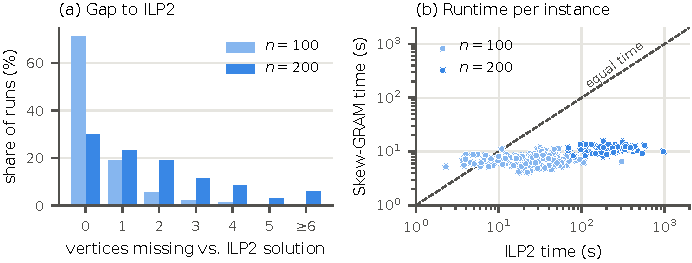
\includegraphics[width=\textwidth]{fig3_results.pdf}
\caption{(a) Number of vertices missing from the Skew-GRAM path compared with the ILP2 solution, over all runs (0: ILP2 length reached or exceeded). (b) Running time per instance (Skew-GRAM: mean over the five seeds); points below the dashed line are faster with Skew-GRAM.}
\label{fig:results}
\end{figure}

Table~\ref{tab:instances} details ten instances, chosen at the 0th, 50th, 80th, 95th and 100th percentiles of the mean gap for each size. With 100 vertices most instances reach the ILP2 length, and the gap is concentrated on a few instances on which the guided walks rarely reach the region of $D$ that contains the best path. With 200 vertices the gaps are larger (up to 8 vertices in a run), while on instance 200\_68 Skew-GRAM exceeds the ILP2 solution in four runs out of five.

\begin{table}[t]
\centering
\caption{Per-instance results for ten instances, chosen at the 0th, 50th, 80th, 95th and 100th percentiles of the mean gap for each size (best first). Skew-GRAM: mean $\pm$ standard deviation over the five seeds. A positive gap means a longer path than the ILP2 solution.}
\label{tab:instances}
% Généré par scripts/make_paper_assets.py — ne pas modifier à la main.
\setlength{\tabcolsep}{7pt}
\begin{tabular}{@{}l S[table-format=2.0] S[table-format=2.1]@{\,$\pm$\,}S[table-format=1.1] S[table-format=-2.1] S[table-format=3.1] S[table-format=2.1]@{}}
\toprule
 & \multicolumn{3}{c}{Length (vertices)} & {Gap} & \multicolumn{2}{c}{Time (s)} \\
\cmidrule(lr){2-4} \cmidrule(l){6-7}
{Instance} & {ILP2} & \multicolumn{2}{c}{Skew-GRAM} & {(\%)} & {ILP2} & {Skew-GRAM} \\
\midrule
100\_4 & 11 & 11.0 & 0.0 & 0.0 & 29.0 & 6.1 \\
100\_230 & 10 & 9.8 & 0.4 & -2.0 & 16.1 & 8.2 \\
100\_133 & 13 & 12.0 & 0.0 & -7.7 & 20.6 & 6.4 \\
100\_247 & 6 & 5.0 & 0.0 & -16.7 & 27.0 & 9.3 \\
100\_300 & 9 & 5.0 & 0.0 & -44.4 & 16.9 & 7.9 \\
\addlinespace
200\_68 & 7 & 9.2 & 1.3 & 31.4 & 183.9 & 11.9 \\
200\_50 & 9 & 7.6 & 1.3 & -15.6 & 134.6 & 9.1 \\
200\_61 & 7 & 5.0 & 0.0 & -28.6 & 440.3 & 12.5 \\
200\_49 & 9 & 5.4 & 0.9 & -40.0 & 225.2 & 11.2 \\
200\_41 & 13 & 7.2 & 1.6 & -44.6 & 108.1 & 12.4 \\
\bottomrule
\end{tabular}

\end{table}

\subsubsection{Stability across seeds.}
The decoder is stochastic, so we measure how results vary with the seed. The mean length over all instances is very stable (standard deviation 0.02 vertex for $n=100$ and 0.12 for $n=200$). At the level of single instances, the length returned for an instance changes with the seed by 0.43 vertex on average (standard deviation) for $n=100$ and 0.93 for $n=200$; the five runs return the same length on 48\,\% and 23\,\% of the instances. The running time of an instance also varies between runs (standard deviation 2.4\,s on average for $n=100$), mostly because the machine was shared with other work: the amount of computation is the same in every run, since the number of walks is fixed. Keeping the best of the five runs would raise the number of instances on which the ILP2 length is reached to 273 of 298 and 42 of 70, at five times the cost.

\subsection{Real Metabolic Networks}
\label{sec:bio}

Table~\ref{tab:bio} reports the results on the 25 KEGG pathways. Skew-GRAM finds the exact optimum on every pathway and with every seed. These instances are much easier than the synthetic ones: they have at most 38 vertices, and $G$ is very sparse (8.7 edges on average), so the optimum is short (3.4 vertices on average) and equals a single vertex for 7 pathways. Exact enumeration with the component cut takes less than 2\,ms per pathway, far less than the 2.9\,s of Skew-GRAM. On such small networks an exact method is the better choice; the experiment shows that the method applies unchanged to real data and returns correct solutions, but it does not demonstrate a speed advantage. Larger real networks, such as genome-scale metabolic networks coupled with protein interaction data, are needed to assess the method in the regime where exact solvers struggle.

\begin{table}[t]
\centering
\caption{Results on 25 KEGG metabolic pathways (five seeds each). LP$(D)$: number of vertices on a longest path of $D$. Optimum: exact optimum by enumeration. Hits: pathways on which Skew-GRAM reaches the optimum (mean over seeds). Lengths are means.}
\label{tab:bio}
% Généré par scripts/make_paper_assets.py — ne pas modifier à la main.
\setlength{\tabcolsep}{5pt}
\begin{tabular}{@{}l c S[table-format=2.1] S[table-format=1.1] S[table-format=2.1] S[table-format=1.2] S[table-format=1.2] c@{}}
\toprule
Pathways & $|V|$ & {$|A|$} & {$|E|$} & {LP$(D)$} & {Optimum} & {Skew-GRAM} & Hits \\
\midrule
Acyclic (19) & 4--15 & 25.9 & 9.1 & 7.5 & 3.58 & 3.58 & 19/19 \\
With 2-cycles (6) & 12--38 & 97.3 & 7.3 & 13.5 & 2.83 & 2.83 & 6/6 \\
\midrule
All (25) & 4--38 & 43.1 & 8.7 & 9.0 & 3.40 & 3.40 & 25/25 \\
\bottomrule
\end{tabular}

\end{table}

\subsection{Ablation of the DAG Lookahead}

To measure the role of the lookahead, we remove the term $\mathrm{lf}(v)/\tau_{lf}$ from $S(u,v)$ and keep everything else unchanged (seed 42). With 100 vertices, the mean length drops from 9.49 to 7.29 vertices ($-23.2$\,\%), paths become shorter on 229 of 298 instances, and the ILP2 length is reached on 47 instances instead of 216. With 200 vertices, the mean length drops from 7.87 to 6.40 ($-18.7$\,\%) and the ILP2 length is reached on 5 instances instead of 24. Embedding similarity alone does not tell the decoder whether a successor leads to a long branch or to a sink; the lookahead provides this information exactly and at linear cost.

\subsection{Scalability}
\label{sec:scaling}

Table~\ref{tab:scaling} shows how the running time grows with $n$ and where it is spent. Walk generation is negligible. Training grows with the size of the walk corpus, which grows with $n$ and with the length of the walks. Decoding takes the largest share at every size, from 91\,\% of the time for $n=100$ to 57\,\% for $n=1000$: its cost is proportional to the number of walks $W$, to the length of each walk, which is bounded by the longest path of $D$, and to the number of successors scored at each step, and the $G$-bonus compares each candidate with the vertices already on the path. With $n=1000$ (about 25{,}000 arcs), one run takes 143\,s on average. No ILP2 solution is available for these sizes, but the number of vertices on a longest path of $D$, LP$(D)$, is an upper bound on the optimum: the paths found contain 33.5 and 72.8 vertices on average for $n=500$ and $n=1000$, against 46.6 and 94.4 for this bound.

\begin{table}[t]
\centering
\caption{Running time per phase and path length as $n$ grows (all instances, five seeds). $|A|$ and LP$(D)$ (vertices on a longest path of $D$) are means over instances; Length: mean $\pm$ standard deviation across seeds of the mean; Total: mean $\pm$ standard deviation over runs.}
\label{tab:scaling}
% Généré par scripts/make_paper_assets.py — ne pas modifier à la main.
\setlength{\tabcolsep}{4pt}
\begin{tabular}{@{}S[table-format=4.0] S[table-format=3.0] S[table-format=5.0] S[table-format=2.1] S[table-format=2.2]@{\,$\pm$\,}S[table-format=1.2] S[table-format=1.2] S[table-format=2.1] S[table-format=2.1] S[table-format=3.1]@{\,$\pm$\,}S[table-format=2.1]@{}}
\toprule
 & & & & \multicolumn{2}{c}{Length} & \multicolumn{5}{c}{Time per run (s)} \\
\cmidrule(lr){5-6} \cmidrule(l){7-11}
{$n$} & {Inst.} & {$|A|$} & {LP$(D)$} & \multicolumn{2}{c}{(vertices)} & {Walks} & {Training} & {Decoding} & \multicolumn{2}{c}{Total} \\
\midrule
100 & 300 & 399 & 15.1 & 9.47 & 0.02 & 0.02 & 0.6 & 6.2 & 6.8 & 2.6 \\
200 & 75 & 999 & 19.6 & 7.83 & 0.15 & 0.06 & 2.6 & 8.6 & 11.3 & 4.2 \\
500 & 10 & 6185 & 46.6 & 33.52 & 1.32 & 0.25 & 19.1 & 29.7 & 49.1 & 8.6 \\
1000 & 5 & 24974 & 94.4 & 72.76 & 1.82 & 0.58 & 60.5 & 81.4 & 142.6 & 13.2 \\
\bottomrule
\end{tabular}

\end{table}

The 30{,}000 walks are the main cost, so we examine how quality depends on $W$. Because the first $k$ walks of a run use exactly the same random numbers as a run with budget $W=k$, the best length after each block of 500 walks gives the result of every smaller budget at no extra cost (Fig.~\ref{fig:budget}). Quality is still increasing at $W=30{,}000$ for every size. With $W=3{,}000$, the paths keep between 79\,\% ($n=500$) and 92\,\% ($n=1000$) of their final length, and the share of runs reaching the ILP2 length falls from 71.3\,\% to 34.4\,\% for $n=100$. Reducing $W$ is therefore not a free saving. Three remedies follow from the structure of the decoder. The walks are independent and can run in parallel. The $G$-bonus can be maintained incrementally by storing the set of $G$-neighbours of the current path, which makes it $O(1)$ per candidate instead of $O(L)$. Finally, the budget could adapt to the instance, for example by stopping when the best length has not improved for a given number of walks. We leave these engineering improvements to future work.

\begin{figure}[t]
\centering
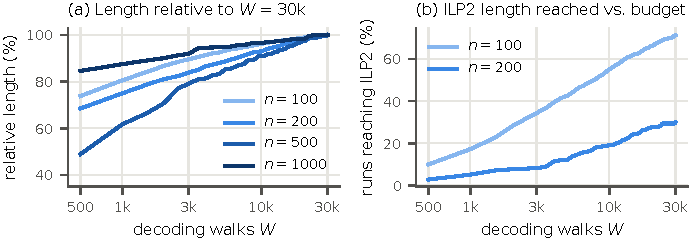
\includegraphics[width=\textwidth]{fig4_budget.pdf}
\caption{Effect of the number of decoding walks $W$. (a) Mean path length relative to the length obtained with $W=30{,}000$. (b) Share of runs that reach the ILP2 length (instances with an ILP2 solution).}
\label{fig:budget}
\end{figure}

\subsection{Discussion and Limitations}

The results support the combination of learned and exact components. The lookahead gives the decoder exact information that is cheap to compute on a DAG, instead of asking the embedding model to learn it. $G$ is used for guidance and for the final check rather than inside the embedding objective, which keeps the learning problem focused on the order of the path, while the extraction step guarantees feasibility.

The method has clear limits. It is a heuristic and should not replace ILP2 when optimality must be guaranteed. Its gap to ILP2 grows with $n$ for a fixed budget, and on small real pathways exact enumeration is both exact and faster. The embeddings are trained for each instance, which adds a training cost that a model trained across instances would avoid. Finally, our real-data evaluation covers small pathways only, and the orientation of reversible reactions is a simplification.

% ============================================================
\section{Conclusion}
% ============================================================

We presented Skew-GRAM, which applies the Skip-Gram model from NLP to the One-to-one SkewGRAM problem from biology: finding a longest path in a DAG whose vertices are connected in a second graph. Embeddings learned from directed random walks guide a Monte-Carlo decoder together with an exact DAG lookahead and a connectivity bonus, and an exact Union-Find step makes every returned path feasible. On 368 synthetic instances with an ILP2 solution, the method reaches the ILP2 length in most runs with 100 vertices and runs much faster than ILP2, with a speedup that grows with the size of the graphs; its average results vary little across seeds, it finds the exact optimum on 25 real metabolic pathways, and it scales to graphs with 1000 vertices. Future work will address larger real networks, a faster decoder (parallel walks, incremental $G$-bonus, adaptive budget) and embeddings trained across instances.

% ============================================================
% REFERENCES (style splncs04)
% ============================================================

\begin{thebibliography}{10}

\bibitem{sidi2022}
Ahmed Sidi, M.L., Bocquillon, R., Mohamed Babou, H., Dhib, C., Néron, E., Soukhal, A., Nanne, M.F.: Improved approaches to solve the one-to-one SkewGraM problem. Computers \& Operations Research \textbf{138}, 105584 (2022)

\bibitem{sidi_dl}
Ahmed Sidi, M.L., Mohamed Babou, H., Dhib, C.: Deep learning approaches for finding a longest DG-consistent path in biological networks. Preprint (2024)

\bibitem{sidi}
Ahmed Sidi, M.L., Mohamed Babou, H., Dhib, C., Néron, E., Soukhal, A., Nanne, M.F.: Constraint programming approaches for finding conserved metabolic and genomic patterns. Computers \& Operations Research \textbf{183}, 107166 (2025)

\bibitem{bellman1958}
Bellman, R.: On a routing problem. Quarterly of Applied Mathematics \textbf{16}(1), 87--90 (1958)

\bibitem{bello2016}
Bello, I., Pham, H., Le, Q.V., Norouzi, M., Bengio, S.: Neural combinatorial optimization with reinforcement learning. arXiv preprint arXiv:1611.09940 (2016)

\bibitem{dai2017}
Dai, H., Khalil, E.B., Zhang, Y., Dilkina, B., Song, L.: Learning combinatorial optimization algorithms over graphs. In: Advances in Neural Information Processing Systems, vol.~30 (2017)

\bibitem{erdos1959}
Erd\H{o}s, P., Rényi, A.: On random graphs I. Publicationes Mathematicae Debrecen \textbf{6}, 290--297 (1959)

\bibitem{fertin2012}
Fertin, G., Mohamed Babou, H., Rusu, I.: Algorithms for subnetwork mining in heterogeneous networks. In: Experimental Algorithms (SEA 2012). LNCS, vol.~7276, pp. 184--194. Springer (2012)

\bibitem{grover}
Grover, A., Leskovec, J.: node2vec: scalable feature learning for networks. In: Proceedings of the 22nd ACM SIGKDD International Conference on Knowledge Discovery and Data Mining, pp. 855--864 (2016)

\bibitem{kanehisa2000}
Kanehisa, M., Goto, S.: KEGG: Kyoto Encyclopedia of Genes and Genomes. Nucleic Acids Research \textbf{28}(1), 27--30 (2000)

\bibitem{karalias2020}
Karalias, N., Loukas, A.: Erd\H{o}s goes neural: an unsupervised learning framework for combinatorial optimization on graphs. In: Advances in Neural Information Processing Systems, vol.~33 (2020)

\bibitem{kingma2014}
Kingma, D.P., Ba, J.: Adam: a method for stochastic optimization. arXiv preprint arXiv:1412.6980 (2014)

\bibitem{mikolov}
Mikolov, T., Sutskever, I., Chen, K., Corrado, G., Dean, J.: Distributed representations of words and phrases and their compositionality. In: Advances in Neural Information Processing Systems, vol.~26 (2013)

\bibitem{perozzi}
Perozzi, B., Al-Rfou, R., Skiena, S.: DeepWalk: online learning of social representations. In: Proceedings of the 20th ACM SIGKDD International Conference on Knowledge Discovery and Data Mining, pp. 701--710 (2014)

\bibitem{sharan2006}
Sharan, R., Ideker, T.: Modeling cellular machinery through biological network comparison. Nature Biotechnology \textbf{24}(4), 427--433 (2006)

\bibitem{tarjan1975}
Tarjan, R.E.: Efficiency of a good but not linear set union algorithm. Journal of the ACM \textbf{22}(2), 215--225 (1975)

\bibitem{vinyals2015}
Vinyals, O., Fortunato, M., Jaitly, N.: Pointer networks. In: Advances in Neural Information Processing Systems, vol.~28 (2015)

\bibitem{zaharia}
Zaharia, A., Labedan, B., Froidevaux, C., Denise, A.: CoMetGeNe: mining conserved neighborhood patterns in metabolic and genomic contexts. BMC Bioinformatics \textbf{20}, 19 (2019)

\end{thebibliography}

% ============================================================
% RESPONSE TO THE REVIEWERS
% ============================================================
\clearpage
\section*{Response to the Reviewers}
\noindent Submission 119, I2COMSAPP'26 --- ``One-to-one SkewGRAM: Applying NLP Embeddings to Biological Graph Optimization''
\medskip

We thank both reviewers for their careful reading and their suggestions. Since the submitted version, the synthetic benchmark has grown from 38 to 375 instances (300 with 100 vertices and 75 with 200 vertices, 368 of them with an ILP2 solution), and every experiment has been repeated with five random seeds. All numbers in the paper were recomputed on this benchmark. The points raised by the reviewers are answered below.

\subsubsection{Reviewer 1.}

\begin{description}
\item[R1.1] \emph{Formatting.} The paper now follows the Springer LNNS template (\texttt{llncs} class): standard author and affiliation block, single-paragraph abstract, references in the Springer style, figures redrawn at the text width with readable fonts, tables rebuilt with aligned columns. The paper fits within the 15-page limit.

\item[R1.2] \emph{Evaluation on real biological networks.} We added an evaluation on 25 real metabolic pathways from KEGG (seven bacteria, Sect.~5.3, Table~4). Since ILP2 solutions are not available for them, we computed their exact optimum by enumeration with two exact cuts. Skew-GRAM finds the exact optimum on all 25 pathways and with all five seeds. We also state the limits of this experiment openly: these pathways are small (at most 38 vertices) and $G$ is very sparse, so exact enumeration is faster than our method on them. The experiment shows that the method applies unchanged to real data and returns correct solutions; assessing it on larger real networks, where exact solvers struggle, is listed as future work.

\item[R1.3] \emph{Scalability and the 30,000 Monte-Carlo walks.} We added a scalability study (Sect.~5.5) on 10 instances with 500 vertices and 5 instances with 1000 vertices. Table~5 breaks the running time down by phase: decoding dominates, and one run on a 1000-vertex graph takes about 143\,s. We also measured how quality depends on the number of walks (Fig.~4); this costs no extra computation, because the first $k$ walks of a run are exactly a run with budget $k$. Quality is still increasing at 30,000 walks, so reducing the budget is not a free saving. We discuss three remedies that follow from the structure of the decoder: running the independent walks in parallel, maintaining the $G$-bonus incrementally, and adapting the budget to the instance.

\item[R1.4] \emph{Standard deviations over multiple runs.} Every instance is now solved with five seeds. Table~2 reports means with their standard deviation across seeds, Table~3 gives the per-instance mean and standard deviation of the path length, and a paragraph on stability across seeds (Sect.~5.2) reports the per-instance variability of lengths and running times.
\end{description}

\subsubsection{Reviewer 2.}

\begin{description}
\item[R2.1] \emph{French text in Figures 1, 4 and 5.} All figures are now in English. Figure~1 was redrawn with a corrected toy example in which the highlighted path is the unique optimum and the longest path of $D$ is infeasible. The two method diagrams were merged into Fig.~2. The result figures (Figs.~3 and~4) were regenerated from the new experiments.

\item[R2.2] \emph{Title.} We adopted the suggested title, ``One-to-one SkewGRAM: Applying NLP Embeddings to Biological Graph Optimization'', which describes the direction of the transfer more accurately.

\item[R2.3] \emph{Real biological networks.} See our answer to R1.2.

\item[R2.4] \emph{Table 2 alignment.} The per-instance table (now Table~3) was rebuilt with decimal-aligned columns, true minus signs and a separate column for standard deviations, so that values no longer run together. It now covers instances of both sizes.
\end{description}

In addition, we corrected the citation of ILP2, which was introduced by Ahmed Sidi et al.\ (Computers \& Operations Research, 2022), and we now state that the DL2 result (1.2 vertices) was reported on a different benchmark of 50-vertex instances and was not re-run. The larger benchmark also revealed that one ILP2 reference solution with 200 vertices is not optimal (Skew-GRAM finds a longer feasible path, which we verified independently); the paper therefore treats ILP2 solutions as reference lengths rather than certified optima.

\end{document}

